\documentclass[a4paper,11pt]{article}

\usepackage[utf8x]{inputenc}
\SetUnicodeOption{mathletters}
\SetUnicodeOption{autogenerated}

\usepackage[italian]{babel}
\usepackage{booktabs}
\usepackage{mathpazo}
\usepackage{graphicx}
\usepackage[left=2cm, right=2cm, bottom=3cm]{geometry}
\frenchspacing

\begin{document}
\noindent {\Large Olimpiadi italiane di informatica 2012 - OII 2012}
\vspace{0.5cm}

\noindent {\Huge Allenamento per la maratona (\texttt{fontane})}


\section*{Descrizione del problema}
  
\textbf{Nota storica:} in pochi sanno che Turing era un patito
maratoneta, a tal punto che il suo record personale, ottenuto il 25
agosto del 1947, 2 ore e 46 minuti e 3 secondi,  è stato di soli 11
minuti superiore a quello del vincitore delle Olimpiadi del 1948
(l'argentino Delfo Cabrera, che vinse in 2 ore, 34 minuti e 51 secondi).

Alan Turing si vuole allenare per la maratona. Il suo problema è quello
di rifornirsi d'acqua. Ha una mappa piuttosto accurata della zona, con
segnate tutte le fontanelle disponibili, e sulla quale ha riportato il
percorso che intende fare. Ha scelto un percorso formato solo da tratti
in direzione orizzontale (Est-Ovest) o verticale (Nord-Sud). Turing, per
semplicità, "consuma" $1$ml di acqua per ogni metro che corre: dopo aver
bevuto $100$ml, per esempio, è in grado di correre per 100 metri. Turing
però non vuole bere mai più di $100$ml per volta, e vuole correre senza
essere appesantito: quindi, vuole portarsi appresso una borraccia più
piccola possibile. Data la mappa con segnate le fontanelle, aiutate
Turing a capire qual è la capacità della più piccola borraccia che gli
consente di correre avendo sempre acqua a sufficienza.
    
\begin{figure}[h!]
  \centering
  \caption{}
  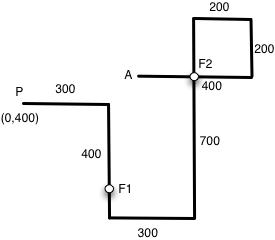
\includegraphics{figura.png}
\end{figure}

Considerate l'esempio mostrato in figura, dove l'origine degli assi
$(0,0)$ è in basso a sinistra: qui Turing parte dal punto di coordinate
$(0,400)$ (marcato da una P) e corre lungo $7$ tratti lunghi, in ordine,
rispettivamente $300$, $400$, $300$, $700$, $200$, $200$ e $400$ metri.
Ci sono due fontanelle nel percorso, la prima (marcata come F1) nel
punto di coordinate $(300,100)$ e la seconda (marcata come F2) nel punto
di coordinate $(600,500)$. Per questo percorso, Turing ha bisogno di una
borraccia da $800$ ml: infatti, partendo con la borraccia piena,
incontra la prima fontanella dopo 600 metri. Qui Turing beve ($100$ml),
e riempie la borraccia ($800$ml), cosa che gli fornisce l'autonomia per
raggiungere la seconda fontanella, che dista $900$m nel percorso da lui
seguito. A questo punto, seguendo il suo percorso, passa nuovamente per
la seconda fontanella dopo $800$m, e da qui gli mancano solo $200$m per
l'arrivo. Come si vede, una borraccia da $800$ml gli è sufficiente per
potersi allenare in questo percorso. 
    
Si assume che Turing parte sempre con la borraccia e la pancia piena.
Nota bene: Turing, oltre a riempire la borraccia, quando arriva a una
fontanella può bere e, in ogni istante, Turing può avere al massimo
$100$ml in pancia: per esempio, se beve $100$ml a una fontana e dopo 20
metri incontra un'altra fontana, a questa può bere solo $20$ml. 
    

\section*{Dati di input}
  
Il file di input consiste di $N+M+2$ righe. La prima riga contiene due
interi $N$ ed $M$, rispettivamente il numero di tratti in cui il suo
percorso è suddiviso, e il numero di fontanelle presenti nella zona.
    
Le successive $N+1$ righe contengono ciascuna due interi $X_{i}$,
$Y_{i}$, le coordinate (in metri) dell'$i$-esimo vertice del percorso di
Turing.
    
Le ultime $M$ righe contengono ciascuna due interi $S_{x}$, $S_{y}$, le
coordinate (in metri) delle fontanelle.
    
L'istanza mostrata nel file di esempio si riferisce a quella mostrata in
figura.
    
\section*{Dati di output}
  
Il file di output consiste di un unica riga contente un unico intero
$T$: la capacità in ml della borraccia che Turing dovrà comprare per
poter completare il suo percorso utilizzando solo i rifornimenti lungo
di esso.
    
\section*{Assunzioni}

\begin{itemize}
  \item $1 ≤ N, M ≤ 100\,000$
  \item $1 ≤ X_{i}$$, Y_{i}$$, S_{x}$$ S_{y}$$ ≤ 10^{9}$
  \item $1 ≤ T ≤ 10^{9}$
\end{itemize}

\section*{Valutazione delle soluzioni}

\begin{itemize}
  \item (SubTask 1 - 5 punti) Questo subtask è costituito da una sola
    istanza: il caso di esempio mostrato qui sotto.
  \item (SubTask 2 - 17 punti) Nelle istanze di questo subtask il
    percorso di Turing è su una linea retta e $N=1$.
  \item (SubTask 3 - 15 punti) Nelle istanze di questo subtask  $N ≤
    100$ e $1 ≤ X_{i}$$, Y_{i}$$, S_{x}$$, S_{y}$$ ≤ 1000$.
  \item (SubTask 4 - 48 punti) Nelle istanze di questo subtask il
    percorso di Turing passa al massimo $5$ volte su ciascuna delle
    fontane.
  \item (SubTask 5 - 7 punti) Nelle istanze di questo subtask il
    percorso di Turing è su una linea retta.
  \item (SubTask 6 - 8 punti) Nelle istanze di questo subtask non ci
    sono vincoli particolari.
\end{itemize}

\section*{Esempi di input/output}
    \noindent
    \begin{tabular}{p{11cm}|p{5cm}}
    \toprule
    \textbf{File \texttt{input.txt}}
    & \textbf{File \texttt{output.txt}}
    \\
    \midrule
    \scriptsize
    \begin{verbatim}
7 2
0 400
300 400
300 0
600 0
600 700
800 700
800 500
400 500
300 100
600 500
      \end{verbatim}
    &
    \scriptsize
    \begin{verbatim}
800
      \end{verbatim}
    \\
    \bottomrule
    \end{tabular}
  
\section*{Nota/e}
\begin{itemize}
  \item Non tutte le fontanelle sono sul percorso seguito da Turing; non
    esistono due fontane nella stessa posizione (ovvero, con le stesse
    coordinate).
  \item Il tratto tra due vertici consecutivi del percorso di Turing è
    sempre in orizzontale o in verticale.
  \item Il percorso di Turing potrebbe utilizzare più di una volta la
    stessa fontanella.
  \item Si assume che Turing parta con la borraccia piena (e la pancia
    piena: $100$ml).
  \item Ci possono essere tratti consecutivi che sono paralleli (sia
    sovrapposti che con lo stesso verso).
\end{itemize}

\end{document}
